% !TEX root = ../../Article.tex
\section{Data Transfer Speed}
\subsection{Description and Motivation}
Transfer speed is a very vital for part of the smart card interaction. If the smart card application or the transportation layer are incaple of handling large amounts of the data we will need to take that into account when examining the usability of smart cards. In order to test and eliminate as many variables as possible the smart card is programmed to receive data, initialize a buffer, copy the incoming data to the buffer and send the exact same data in return. Figure \ref{fig:nfcDataflowTest} describes this process using an NFC card as a platform for the Java Card Applet.

\begin{figure}[h!]
  \caption{Data flow of data transfer speed test for NFC.}
  \label{fig:nfcDataflowTest}
  \centering
    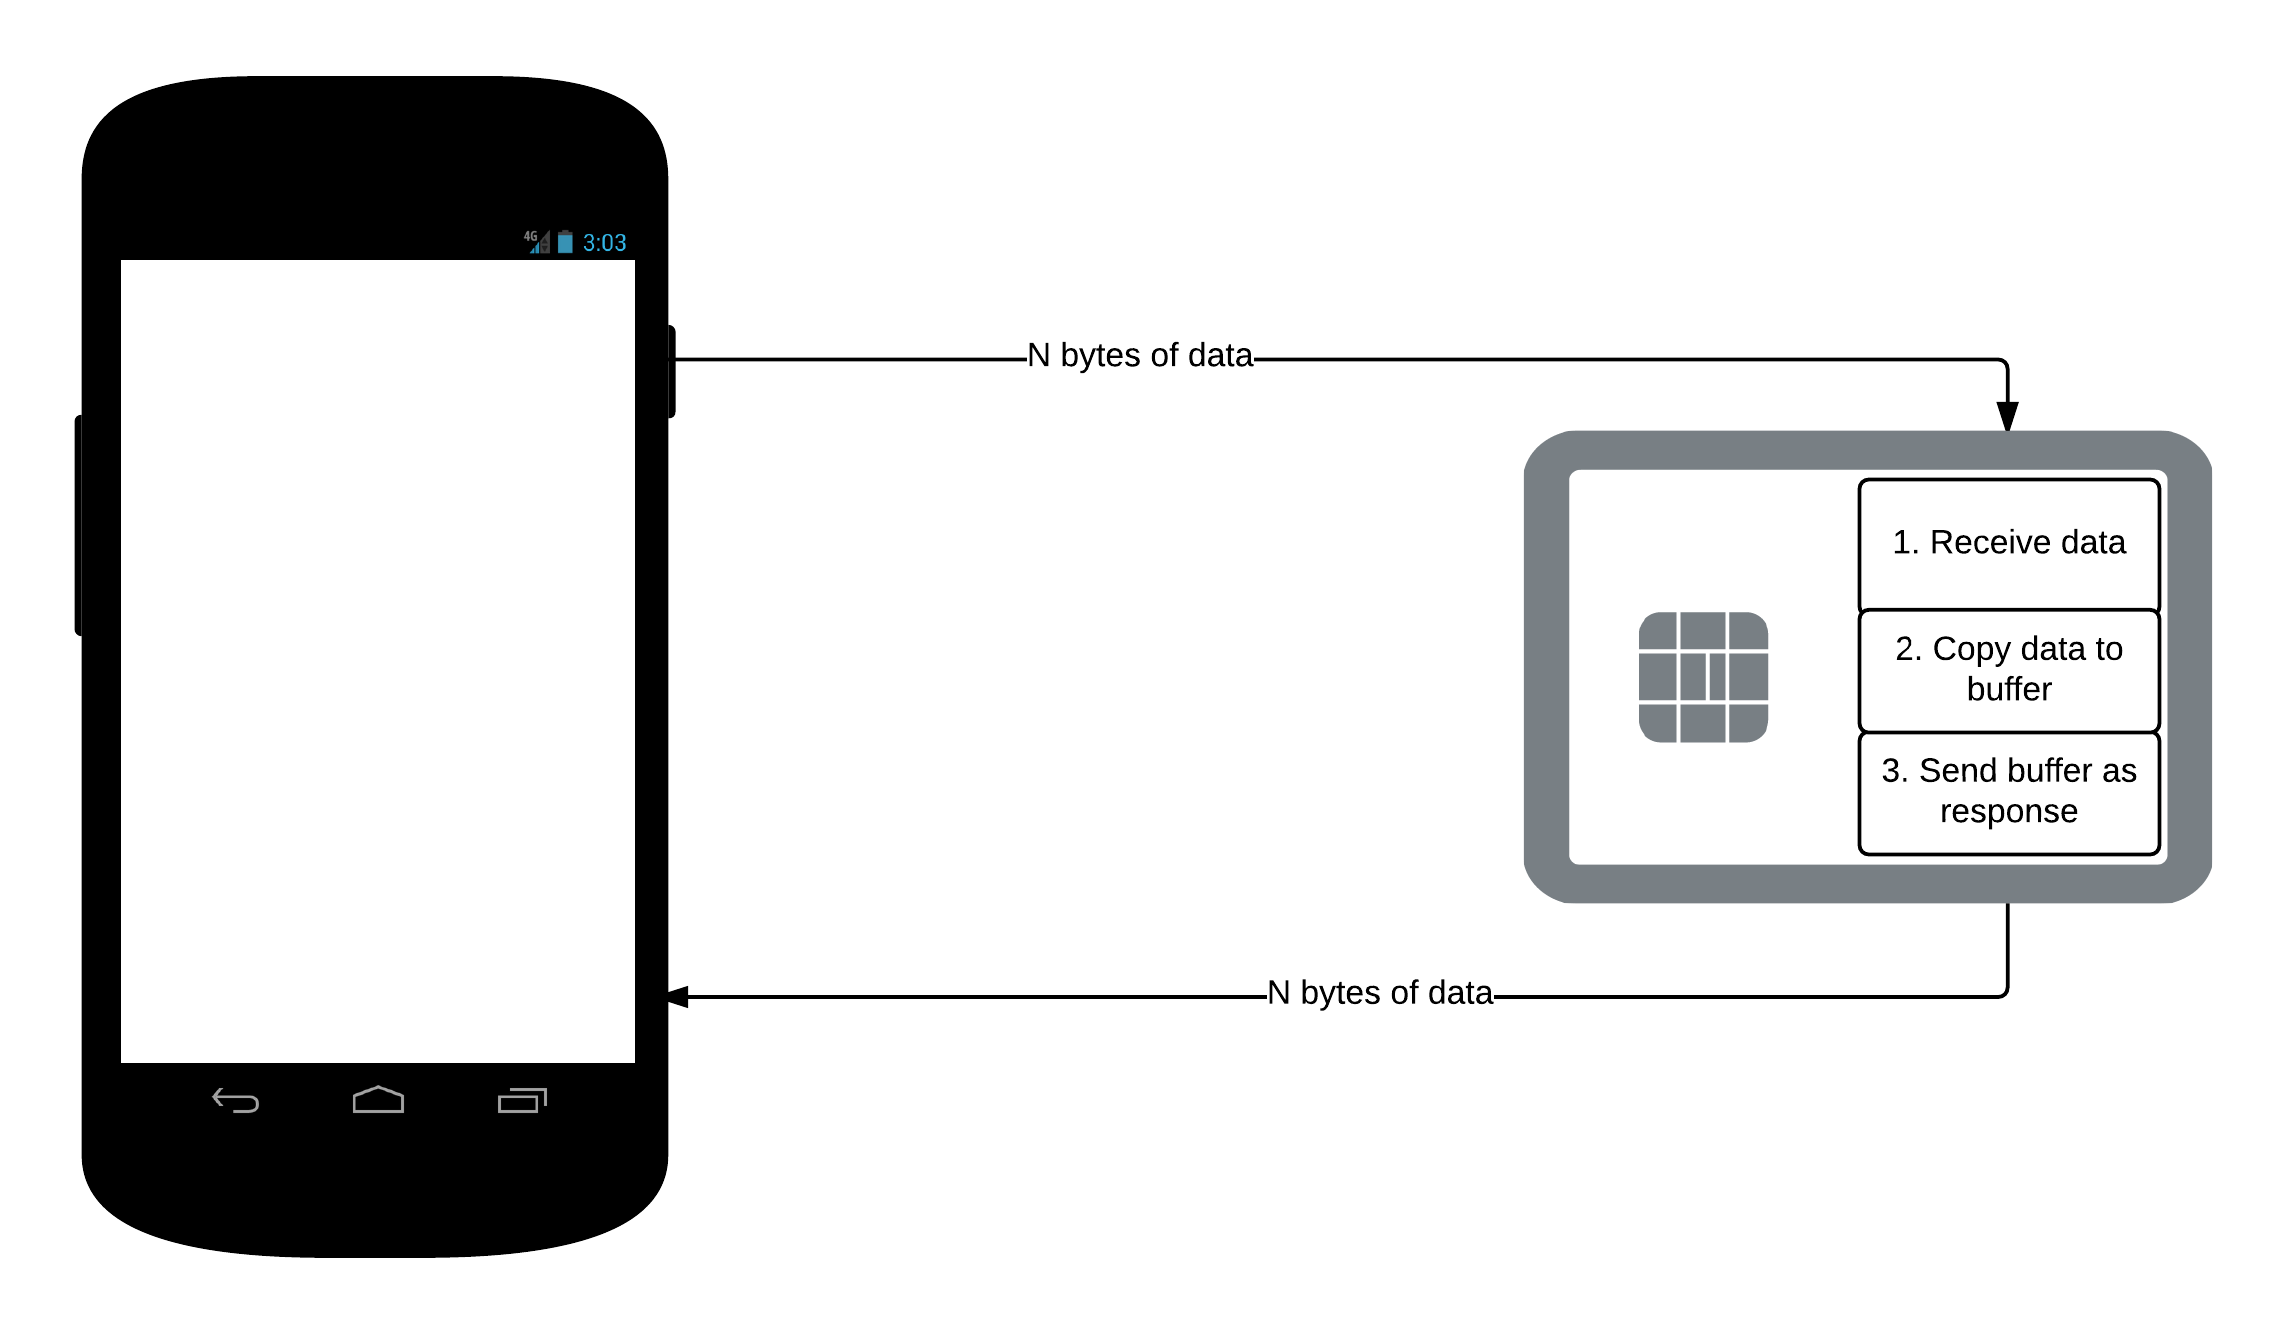
\includegraphics[width=0.95\textwidth]{images/NFCTransferTest.png}
\end{figure}

\subsection{Tests and Results}
\paragraph{NFC}\mbox{}\\
\begin{table}[h!]
\caption{Table of NFC transfer speed test.}
\label{tbl:nfcspeed}
\centering

    \begin{tabular}{ | l | r | r | r |}
        \hline
        \thead{Data size (byte)}
        & \thead{T1}
        & \thead{T2}
        & \thead{T3} \\ \hline

        10000 & 3,8s & 4,1s & 3,6s \\ \hline
        100000 & 41,3s & 35,0s & 24,7s \\ \hline
        1000000 & 602,1s & 361,3s & 235,1s \\ \hline

    \end{tabular}

\end{table}

%\vspace{1cm}
\begin{figure}[h!]

    \caption{Graphical representation of table \ref{tbl:nfcspeed}.}
    \label{fig:nfcgraph}
    \begin{tikzpicture}
        \centering
            \begin{axis}[
                width  = 0.85*\textwidth,
                height = 8cm,
                major x tick style = transparent,
                ybar=2*\pgflinewidth,
                bar width=14pt,
                ymajorgrids = true,
                ylabel = {Running time (seconds)},
                xlabel = {Data size (byte)},
                symbolic x coords={10000, 100000, 1000000},
                xtick = data,
                scaled y ticks = false,
                enlarge x limits=0.25,
                ymin=0,
                legend cell align=left,
                legend style={
                        at={(1,1.05)},
                        anchor=south east,
                        column sep=1ex
                }
            ]
                \addplot[style={bblue,fill=bblue,mark=none}]
                    coordinates {(10000, 3.89) (100000, 41.29) (1000000, 602)};

                \addplot[style={rred,fill=rred,mark=none}]
                     coordinates {(10000, 4) (100000, 35) (1000000, 361)};

                \addplot[style={ggreen,fill=ggreen,mark=none}]
                     coordinates {(10000, 3.6) (100000, 24) (1000000, 235)};

                \legend{T1 Configuration,T2 Configuration,T3 Configuration}


            \end{axis}
    \end{tikzpicture}
\end{figure}


\newpage
\paragraph{Micro SD}\mbox{}\\
T1 configuration, from NFC was dropped when testing transfers speed for micro SD as it became clear from previous tests on NFC that T1 is vastly inferior to T2 and T3. A non-asyncronous (not using streams) Android application is not representative of the "real-world" and we decided on not pursuing further test results using this configuration.

T2 configuration consist of the Android application sending data to the smart card application using frames of size 255 byte until all data is sent. Simultaneously the responses are written to an internal file using FileOutputStream (provided by the standard Java library).

We were not able to test T3 configuration as explained in section \ref{sec:limitationsMSD}.

\begin{table}[h!]
\caption{Table of micro SD transfer speed test.}
\label{tbl:msdspeed}
\centering

    \begin{tabular}{ | l | r | r |}
        \hline
        \thead{Data size (byte)}
        & \thead{T2}
        & \thead{T3} \\ \hline

        10000  & 3,18s & N/A s \\ \hline
        100000 & 16,14s & N/A s \\ \hline
        1000000 & 142s & N/A s \\ \hline

    \end{tabular}

\end{table}


\newpage
\subsection{Conclusion}
From table \ref{tbl:nfcspeed} and figure \ref{fig:nfcgraph} we can learn that we are able to optimize the data transfer and processing speed between the Android application and the NFC card. It is also clear that when we are transmitting low amounts there are virtually no difference between the configurations; T1, T2 and T3. The differences are more prominent when the data amounts increases. Even though we achieved an improvement of approximately 60 \% from T1 to T3 when sending 1 MB of data, the process is still time consuming.

If we compare the test results for T2 configuration on the NFC card and micro SD card we can clearly see an improvement on the micro SD card. The micro SD card had a ~60 \%  better running time over the NFC card when sending 1 MB of data. Although we were not able to test configuration T3 on the micro SD card, results point in the direction of micro SD cards having better performance than NFC cards.

Even though we are able to optimize and improve data transfer speeds, we are still very far from transferring and processing large amounts of data quickly. We have to take this into account when evaluating areas of use for the smart card. Transfer and processing speed rules out many areas concerning large amounts of data, such as full data encryption.
